\chapter{Maintaining a Healthy Work-Life Environment}

The lecture is brief, but its order is exact. We begin with a managerial question, not with a doctrine of culture. The speaker first appeals to what repeated interviews reveal, then widens that evidence into a diagnosis of the last decade, then shows what changed when times became turbulent and COVID interrupted routine. Only after that do we see why perks are a weak answer and why care and trajectory become the decisive terms. There is no validated blackboard mathematics to preserve here, so the formalism below is a cautious reconstruction of the spoken mechanism.

\section{The Question and the Evidence of Interviews}

The opening question is straightforward: what does one do to maintain a healthy work-life environment? The answer begins with observation. The speaker says, in effect, that interviewing many people lets us see two things at once: why they are leaving companies, and what they are looking for next. That is the empirical base of the chapter.

\begin{definition}
Let \(I\) denote the evidence supplied by repeated interviews with employees and candidates. We write \(M\) for relatively easy market conditions, \(W\) for compensation that is sufficiently attractive to keep people in place, \(T\) for turbulence, \(P\) for perks, \(C\) for perceived care from the company, \(G\) for room to grow and develop, and \(R\) for willingness to stay.
\end{definition}

The important point is methodological. The lecture does not begin by saying what culture ought to be. It begins by asking what patterns become visible when many workers explain their exits. In that sense the argument is diagnostic before it is prescriptive.

\begin{remark}
The symbols in this chapter are not quoted from a board. They are a compact notation for a verbal argument whose structure is already clear in the transcript.
\end{remark}

\section{Why the Old Regime Could Persist}

From interview evidence the speaker pivots to a broader historical claim. For about a decade, many companies could treat people impersonally and still retain them. The reason was not that such treatment had become healthy; the reason was that pay and general conditions were strong enough to hide the weakness.

\begin{equation}
M \uparrow \land W \uparrow \;\Rightarrow\; R \text{ may remain high even when } C \downarrow .
\end{equation}

This is the first real structural move of the lecture. We must distinguish between observed retention and a genuinely healthy environment. A firm can keep people for a time without treating them well. In easy periods, retention is therefore an ambiguous indicator. It may record culture, but it may also record the fact that market conditions and compensation are carrying more weight than the culture deserves.

\section{Turbulence Changes the Question}

The next pivot is the decisive one: what happens when times become turbulent? The speaker's answer is that people ``start waking up.'' We may write that transition schematically as

\begin{equation}
T \uparrow \;\Rightarrow\; E \uparrow ,
\end{equation}

where \(E\) denotes reevaluation. The lecture is careful here in spirit, even if it is quick in form. Turbulence does not create dissatisfaction from nothing. Rather, it removes the cover under which dissatisfaction had been tolerated.

\subsection{Question \& Answer}

\paragraph{Question.} Why should employees reconsider their jobs in turbulent times if they tolerated those same jobs during the easier period?

\paragraph{Answer.} Because the easier period masked what turbulence exposes. Once routine is broken, workers stop running on inertia and begin inspecting the job itself. The logic may be written as a short chain:

\begin{align}
M \uparrow \land W \uparrow &\Rightarrow \text{weak culture may be masked},\\
T \uparrow &\Rightarrow E \uparrow,\\
E \uparrow &\Rightarrow \text{workers begin to inspect the job directly.}
\end{align}

So the lecture's claim is not that people suddenly become irrationally restless. It is that changing conditions force an audit. A culture that looked adequate while the market was easy may fail that audit once people ask what sort of life the job is actually producing.

\begin{figure}
\centering
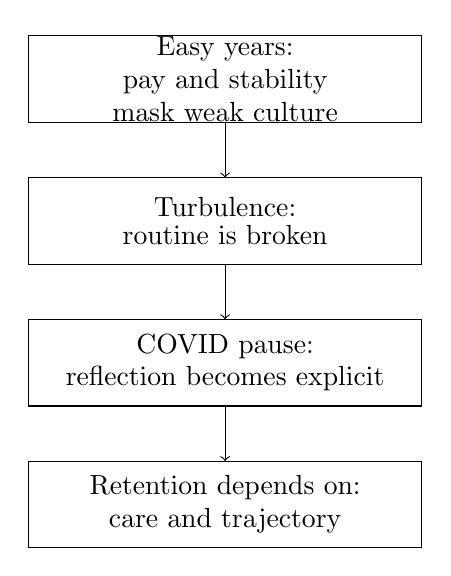
\begin{tikzpicture}[x=1cm,y=1cm]
\draw (0,0) rectangle (5,1.1);
\node at (2.5,0.55) {\shortstack{Easy years:\\pay and stability\\mask weak culture}};
\draw[->] (2.5,0)--(2.5,-0.7);
\draw (0,-1.8) rectangle (5,-0.7);
\node at (2.5,-1.25) {\shortstack{Turbulence:\\routine is broken}};
\draw[->] (2.5,-1.8)--(2.5,-2.5);
\draw (0,-3.6) rectangle (5,-2.5);
\node at (2.5,-3.05) {\shortstack{COVID pause:\\reflection becomes explicit}};
\draw[->] (2.5,-3.6)--(2.5,-4.3);
\draw (0,-5.4) rectangle (5,-4.3);
\node at (2.5,-4.85) {\shortstack{Retention depends on:\\care and trajectory}};
\end{tikzpicture}
\end{figure}

\section{COVID and the Pause of Reflection}

The lecture then makes the mechanism concrete. COVID is introduced not as a general social theory, but as a pause. Work was interrupted, normal momentum slowed down, and that pause gave people time to ask questions that had previously remained implicit.

We can represent that reflective question set as
\begin{align}
\mathcal{Q} = \{&
\text{Why do I do what I do?},\nonumber\\
&\text{Do I actually like my job?},\nonumber\\
&\text{Am I happy where I'm at?}\}.
\end{align}

The lecture's causal claim is then

\begin{equation}
T_{\text{COVID}} \;\Rightarrow\; \mathcal{Q}.
\end{equation}

This is the point at which the argument becomes more personal and more exact. The speaker does not leave the reevaluation in abstract language. He gives its inner content. Workers ask whether they like the work, whether the job fits their life, and whether the life attached to the job is improving. That set of questions prepares the critique of the conventional corporate answer.

\section{Perks Are Not the Main Mechanism}

Many firms, and especially many tech firms, thought they could hold workers by offering free food and similar benefits. The lecture rejects this as the main explanation of retention.

\begin{equation}
P \not\Rightarrow R .
\end{equation}

The force of this statement must be read correctly. It does not say that perks have no value at all. It says that perks are not sufficient. Once workers are asking the first-order questions collected in \(\mathcal{Q}\), conveniences do not answer them. A snack program may improve the day. It does not by itself tell a worker that the company cares for him or her as a person, nor does it demonstrate that life and trajectory are improving.

This gives the lecture a sharp contrast:
\begin{itemize}
\item A perk-first model tries to hold people by adding convenience and surface benefit.
\item The model defended by the lecture tries to hold people by changing the quality of treatment and the direction of development.
\end{itemize}

We can therefore state the lecture's negative lesson in plain form: perks can decorate a weak culture, but they cannot substitute for a healthy one.

\section{Care, Growth, and Trajectory}

Now the lecture reaches its positive answer. People mainly care about two connected things. First, they want to know that the company cares for them as persons. Second, they want actual room to grow and develop, so that their life trajectory is getting better rather than merely remaining tolerable.

For a compact mnemonic we define
\begin{equation}
S_{\text{stay}} = C + G .
\end{equation}

This is not an empirical law with measured coefficients. It is a note-writing device that preserves the speaker's pairing of care and growth. In that notation the lecture's final implication becomes

\begin{equation}
C \uparrow \land G \uparrow \;\Rightarrow\; R \uparrow .
\end{equation}

If we want a slightly broader wrapper without pretending to more precision than the lecture provides, we may write
\begin{equation}
\Pr(\text{stay}) = F(C,G,W,P;T),
\end{equation}
with the explicit caution that the lecture supplies no functional form. Its substantive point is only that, once turbulence has increased and reflection has begun, \(C\) and \(G\) matter more deeply than \(P\).

\paragraph{Worked example.} Let us freeze compensation and turbulence and compare two stylized firms. Firm \(A\) is rich in perks but poor in care and development; Firm \(B\) is the reverse:
\begin{align}
A &: (C,G,P) = (1,1,3),\\
B &: (C,G,P) = (3,3,1).
\end{align}
Then the mnemonic score gives
\begin{align}
S_{\text{stay}}(A) &= C_A + G_A = 1+1 = 2,\\
S_{\text{stay}}(B) &= C_B + G_B = 3+3 = 6.
\end{align}

No numerical measurement is being claimed here. The example serves only to compress the lecture's logic into a usable comparison. Once people are asking whether the job is meaningful and whether life is improving, the care-growth firm dominates the perk-heavy firm.

We may now gather the whole argument into one aligned chain:
\begin{align}
M \uparrow \land W \uparrow &\Rightarrow \text{retention may look strong despite weak care},\\
T \uparrow &\Rightarrow E \uparrow,\\
T_{\text{COVID}} &\Rightarrow \mathcal{Q},\\
P \not\Rightarrow R,\\
C \uparrow \land G \uparrow &\Rightarrow R \uparrow .
\end{align}

The lecture is short, but the spine is clean: easy years hide the problem, turbulence reveals it, perks fail to solve it, and care plus trajectory become the real basis of retention.

\section{Summary}

The lecture unfolds in a deliberate order. It begins with the question of how to maintain a healthy work-life environment, then grounds the answer in what repeated interviews reveal about why people leave and what they seek. From there it explains why impersonal firms could survive for years: compensation and market ease masked the weakness. Turbulence, and then specifically the COVID pause, caused workers to reevaluate their jobs in explicit personal terms. At that point perks were exposed as a shallow answer. The chapter ends where the lecture ends: retention is strongest when the company cares for people as people and when workers can see real growth in their trajectory.